\documentclass[11pt,oneside,a4paper]{memoir}
\usepackage{fontspec}
\usepackage{tabu}
\usepackage{graphicx}
\usepackage{longtable}
\usepackage{multirow}
\usepackage{capt-of}
\usepackage[final]{listings}
\usepackage[unicode=true,xetex,colorlinks=true,linkcolor=blue,urlcolor=blue,bookmarksnumbered=true,bookmarksdepth=3]{hyperref}
\usepackage{bidi} % Must be last



%%%%%%%%%%%%%%%%%%%%%%%%%%%%%%%%%%%%%%%%%%%%%%%%%%%%%%%
%%%%%%%%%%%%%%%%%%%% Configuration %%%%%%%%%%%%%%%%%%%%
%%%%%%%%%%%%%%%%%%%%%%%%%%%%%%%%%%%%%%%%%%%%%%%%%%%%%%%

%%% Fonts %%%
\setmainfont[Ligatures=TeX]{Linux Libertine O}
\newfontfamily{\ezr}[Script=Hebrew]{EzraSIL}

\newfontfamily{\mainnolig}{Linux Libertine O}
\newcommand{\q}{{\mainnolig '}}


%%% Page layout %%%
\settypeblocksize{247mm}{160mm}{*}
\setlrmargins{*}{*}{1}
\setulmargins{*}{*}{1}
\checkandfixthelayout

%%% Hyperref (Information in PDF) %%%
\hypersetup{
unicode=true,
pdfauthor={Claus Tøndering},
pdftitle={Bible Online Learner: Localization Guide}
}

%%% Section numbering %%%
\setsecnumdepth{section}

%%% Lists %%%
\tightlists

%%% listings %%%
\lstset{frame=tb,
  aboveskip=3mm,
  belowskip=3mm,
  showstringspaces=false,
  keepspaces=true,
  columns=flexible,
  basicstyle={\footnotesize\ttfamily},
  numbers=none,
  numberstyle=\tiny\color{gray},
  breaklines=true,
  breakatwhitespace=true,
  tabsize=3,
  captiondirection=LTR  % Required by bidi package (although its documentation says otherwise)
}

\renewcommand{\lstlistingname}{\textsc{Listing}}


%%% Chapter style %%%

% My own version of the ell chapter style:
\makechapterstyle{claus}{%
  \chapterstyle{default}
  \renewcommand*{\chapnumfont}{\normalfont\HUGE\sffamily}
  \renewcommand*{\chaptitlefont}{\normalfont\huge\sffamily}
  \settowidth{\chapindent}{\chapnumfont 111}
  \renewcommand*{\chapterheadstart}{\begingroup
    \vspace*{\beforechapskip}%
    \begin{adjustwidth}{}{-\chapindent}%
    \hrulefill
    \smash{\rule{0.4pt}{15mm}}
    \end{adjustwidth}\endgroup}
  \renewcommand*{\printchaptername}{}
  \renewcommand*{\chapternamenum}{}
  \renewcommand*{\printchapternum}{%
    \begin{adjustwidth}{}{-\chapindent}
    \hfill
    \raisebox{10mm}[0pt][0pt]{\chapnumfont\ifanappendix Appendix\else Chapter\fi\ \thechapter}%
                              \hspace*{1em}
    \end{adjustwidth}\vspace*{-3.0\onelineskip}}
  \renewcommand*{\printchaptertitle}[1]{%
    \vskip\onelineskip
    \raggedleft {\chaptitlefont ##1}\par\nobreak}}

% Default style should still use this font:
\renewcommand*{\chaptitlefont}{\normalfont\huge\sffamily}


%%% Auxiliary tabu environments %%%
\tabulinesep=_2mm %Works together with the \addlinespace[...] values below

\newenvironment{my-longtabu}[2]{
%\begin{center}
\begin{longtabu*}{@{}#1@{}}
  \toprule
  #2\\\addlinespace[-1mm]
  \midrule
  \endhead

  \emph{\rmfamily\normalsize(Continued...)} & \\
  \endfoot

  \addlinespace[-1mm]\bottomrule
  \endlastfoot
}{%
\end{longtabu*}
%\end{center}%
}

\newcommand{\headii}[2]{\textbf{#1} & \textbf{#2}}
\newcommand{\headiii}[3]{\textbf{#1} & \textbf{#2} & \textbf{#3}}


\newenvironment{my-tabu}[2]{%
\begin{center}
\begin{tabu}{@{}#1@{}}
  \toprule
  #2\\\addlinespace[-1mm]
  \midrule
}{%
\addlinespace[-1mm]\bottomrule
\end{tabu}
\end{center}%
}


%%% Allow extra space between words %%%
\sloppy


%%% Font matter %%%
\title{Bible Online Learner:\\Localization Guide}
\author{Claus Tøndering\\Ezer IT Consulting}
\date{21 May 2015}

%\makeindex


\begin{document}
\begin{titlingpage*}
\maketitle

\begin{center}
Copyright © 2015 by Claus Tøndering, claus@ezer.dk

\vspace{5mm}

The document is made available under a Creative Commons Attribution 4.0 International License

(see \url{http://creativecommons.org/licenses/by/4.0/})
\end{center}
\end{titlingpage*}


\clearpage
\tableofcontents
\chapterstyle{claus} % TOC should be in default style. "claus" style starts here.

%%%%%%%%%%%%%%%%%%%%%%%%%%%%%%%%%%%%%%%%%%%%%%%%%%%%%%
%%%%%%%%%%%%%%%%%%%% Introduction %%%%%%%%%%%%%%%%%%%%
\chapter{Introduction}

This document tells you how to create a translation of the user interface of Bible Online Learner
(Bible OL).

You are expected to be familiar with the way Bible OL is used, both by teachers and by students.

\section{Requirements}

Before you start, you must have a copy of the following files:

\begin{verbatim}
class_lang.php
common_lang.php
ETCBC4.en.prop.json
ETCBC4-translit.en.prop.json
file_manager_lang.php
font_lang.php
form_validation_lang.php
intro_text_lang.php
js_lang.php
login_lang.php
menu_lang.php
nestle1904.en.prop.json
privacy_lang.php
shebanq_lang.php
statistics_lang.php
text_lang.php
userclass_lang.php
users_lang.php
\end{verbatim}

These files are so-called ``flat'' text files. This means that they contain no formatting. When you
edit them, you must use a proper text editor, not a word processor such a Microsoft Word. Many text
editors are available. On computers running Windows, the \emph{Notepad} program can be used, although
it has an annoying tendency to add ``.txt'' to the end of file names.

It is preferable that your text editor can read and write text using the UTF-8 encoding. In Windows
Notepad you can select the text encoding in the ``Save As'' dialog.




%%%%%%%%%%%%%%%%%%%%%%%%%%%%%%%%%%%%%%%%%%%%%%%%%%%%%%%%%%%
%%%%%%%%%%%%%%%%%%%% Editing PHP Files %%%%%%%%%%%%%%%%%%%%
\chapter{Editing PHP Files}

Most of the files have file names that end in ``.php''. These are files that provide translations
for the parts of the system that are not directly linked to a Greek or Hebrew database.

A typical entry in one of the PHP files looks like this:

\begin{lstlisting}
$lang['file_exists_overwrite'] = 'The file already exists. Do you want to replace it?';
\end{lstlisting}

When making your translation, you must not change anything to the left of the equals (=) sign. The
text to the right of the equals sign is the translation. As shown above, it must be enclosed in
single quotation marks (\verb|'|) and end with a semicolon.

So if you are making a translation into French, you should change the above line to something like:

\begin{lstlisting}
$lang['file_exists_overwrite'] = 'Le fichier déjà existe. Voulez-vous le remplacer?';
\end{lstlisting}

You are allowed to break the lines and insert extra spaces if you need to; it makes no difference to
the displayed text. So the following entry would also be fine:

\begin{lstlisting}
$lang['file_exists_overwrite'] = 'Le fichier déjà existe.
                                  Voulez-vous le remplacer?';
\end{lstlisting}

There is, however, a few cases where line breaks and spaces must not be inserted. This is described
in Section \ref{sec-email-text}.

In some cases the translation is followed by the characters \verb|//| and some text. This is a
comment that may provide you with additional information. You need not translate it. For example:

\begin{lstlisting}
$lang['user_profile_deleted'] = 'User Profile Deleted'; // Text in title bar
\end{lstlisting}

Here the comment ``Text in title bar'' indicates the reason why the English words are capitalized.
This is irrelevant in languages that do not use upper case in titles.

\section{Special Characters}

\subsection{Punctuation Marks}

If the English string contains punctuation marks -- in particular if it ends with a colon -- you should
include similar punctuation in your own language if it makes sense. Be particularly conscious about
quotation mark styles, which can very greatly from language to language:

\begin{itemize}
\item[] English: ``abc'' or `abc'
\item[] German: »abc« or ,,abc``
\item[] French: « abc »
\end{itemize}

But regardless of your language, the translated string must be enclosed in single quotation marks (\verb|'|) and end
with a semicolon (\verb|;|).


\subsection{Apostrophe or Quotation Mark}

If you need to include the character \verb|'| in the text, you must precede it with the character
\verb|\|. This tells the system that the \verb|'| does not end the string. For example:


\begin{lstlisting}
$lang['dont_care'] = 'Don\'t care';
\end{lstlisting}

\subsection{HTML Code}

In a few places the translated string may contain HTML commands. For example:

\begin{lstlisting}
$lang['select_number_preset'] = 'Select number of questions<br>using preset passages';
\end{lstlisting}

HTML commands are enclosed in \verb|<| and \verb|>| characters. You should not change them in the
translation.

\subsection{\%s, \%d, and \{0\}}

In some cases the system needs to insert a value into the text string. This may, for example, be the
name of a file. Such values are indicated by \verb|%s|, \verb|%d|, or \verb|{0}| in the text
strings. For example:

\begin{lstlisting}
$lang['user_name_used'] = 'The user name "%s" is already in use';
\end{lstlisting}

or
\begin{lstlisting}
$lang['use_qo_selection'] = 'Do you also wish to use {0} for sentence unit selection?';
\end{lstlisting}

Be sure to include the \verb|%s|, \verb|%d|, or \verb|{0}| in the translated string to indicate
where the system should insert a value.

\section{Email Text}\label{sec-email-text}

A few of the text strings are not displayed on web pages but are sent to users in emails. The rules
for writing these translations are a little different:

\begin{enumerate}
\item The strings are delimited by double quotes (\verb|"|) rather single quotes (\verb|'|).
\item If you need to break a line in the PHP file, you must end the first line with a double quote
  and start the second line with a period followed by a double quote.
\item If you want a line break in the email you must write the string \verb|\n| at the place where
  the line break is needed.
\end{enumerate}

The following example illustrates these three rules:

\begin{lstlisting}
$lang['email_text'] = "This is the text of an "
                      . "email.\nThis is on a "
                      . "new line.\n";
\end{lstlisting}

This will cause the actual text of the email to be:

\begin{verbatim}
        This is the text of an email.
        This is on a new line.
\end{verbatim}

(Strictly speaking, the reason double quotes are used instead of single quotes is that \verb|\n| does not work
within single quotes.)

\section{Overview of the PHP Files}

The following table lists the name of each PHP file an gives a little information about which parts
of the program uses the translations is each file.

\begin{my-longtabu}{>{\footnotesize\ttfamily}lX}{ \headii{\normalsize\textrm{File}}{Examples of use} }
class\_lang.php & Class management under the ``Classes'' menu item.\\

common\_lang.php & Strings used in many different parts of the system.\\

file\_manager\_lang.php & Exercise management under the ``Manage exercises'' menu item.\\

font\_lang.php & Font management under the ``Font preferences'' menu item.\\

form\_validation\_lang.php & Error messages for data input forms.\\

intro\_text\_lang.php & Front page text.\\

js\_lang.php & Text display, exercise editing, exercise execution.\\

login\_lang.php & Login mechanism.\\

menu\_lang.php & The menus.\\

privacy\_lang.php & Privacy statement.\\

shebanq\_lang.php & Strings used when importing queries from SHEBANQ.\\

statistics\_lang.php & Statistics display under the ``Statistics'' menu item.\\

text\_lang.php & Text and exercise display.\\

userclass\_lang.php & Management of a user's membership of a class.\\

users\_lang.php & User management under the ``Users'' menu item.\\

\end{my-longtabu}

The listed examples of use are not exhaustive.


%%%%%%%%%%%%%%%%%%%%%%%%%%%%%%%%%%%%%%%%%%%%%%%%%%%%%%%%%%%%
%%%%%%%%%%%%%%%%%%%% Editing JSON Files %%%%%%%%%%%%%%%%%%%%
\chapter{Editing JSON Files}

A few of the files have file names that end in ``.json''. These are files that provide translations
for the grammatical terms that relate directly to the Hebrew and Greek databases. The format of
these files is completely different from the format of the PHP files.

A typical section in one of the JSON files might look like this:

\begin{lstlisting}
   "part_of_speech_t": {
       "prps": "Personal pronoun",
       "verb": "Verb",
       "adjv": "Adjective"
   },
\end{lstlisting}

When making your translation, you must not change anything to the left of a colon (:). The
text to the right of the colon is the translation. As shown above, it must be enclosed in
double quotation marks (\verb|"|) and end with a comma. If, however, the following line starts with
a \verb|}|, the comma \emph{must} be omitted, as illustrated with the string \verb|"Adjective"| above.

So if you are making a translation into French, you should change the above lines to something like:

\begin{lstlisting}
   "part_of_speech_t": {
       "prps": "Pronom personnel",
       "verb": "Verbe",
       "adjv": "Adjectif"
   },
\end{lstlisting}

\section{Sorting Information}

In the above example the values of the type \emph{part\_of\_speech\_t} have English translations
such as ``Personal pronoun'', ``Verb'', and ``Adjective'' (and several others that were omitted above).

When these values are displayed by the system, they are normally sorted alphabetically:

\begin{center}
  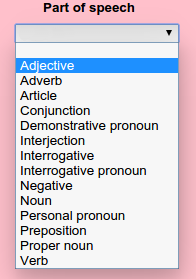
\includegraphics[width=0.3\textwidth]{psp.png}
\end{center}

But sometimes you want another sorting order. If the translation starts with ``\#1'', ``\#2'' etc.
these numbers indicate the sort order. For example:

\begin{lstlisting}
   "gender_t": {
       "f": "#2 Feminine",
       "m": "#1 Masculine",
       "NA": "#3 None",
       "unknown": "#4 Unknown"
   },
\end{lstlisting}

Here, the strings ``\#1'', ``\#2'', etc. indicate the sorting order. Thus:

\begin{center}
  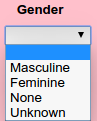
\includegraphics[width=0.148\textwidth]{gender.png}
\end{center}

Be aware that the preferred sorting order in English may not be the preferred sorting order in your language.

\section{Overview of the JSON Files}

The following table lists the JSON files.

\begin{my-tabu}{>{\footnotesize\ttfamily}lX}{ \headii{\normalsize\textrm{File}}{Use} }
ETCBC4.en.prop.json & Grammatical terms for the Hebrew Old Testament.\\
ETCBC4-translit.en.prop.json & Grammatical terms for the transliterated version of Hebrew Old
Testament. (The contents of this file is very similar to the preceding file.)\\
nestle1904.en.prop.json & Grammatical terms for the Greek New Testament.\\
\end{my-tabu}

%%%%%%%%%%%%%%%%%%%%%%%%%%%%%%%%%%%%%%%%%%%%%%%%%%%%%%%
%%%%%%%%%%%%%%%%%%%% Final Actions %%%%%%%%%%%%%%%%%%%%
\chapter{Final Actions}

When you have edited all the files, you must send them to me at claus@ezer.dk. I will then enter
them into the system and you can verify that they are correct. Unfortunately, there is no way for
you to see the result before I have installed the files.

Please be aware that Bible OL is a dynamic program whose features change frequently. As new features
are added to the system, I will contact you and ask you to translate text for the new features.


\end{document}

% Local Variables:
% mode: latex
% ispell-dictionary: "british-ize"
% ispell-extra-args: ("--home-dir=/home/claus/Projects/BibleOL/techdoc")
% eval: (auto-fill-mode 1)
% End:
